% \begin{figure}[t]
%     \centering
%     \begin{minipage}[t]{0.58\linewidth}
%         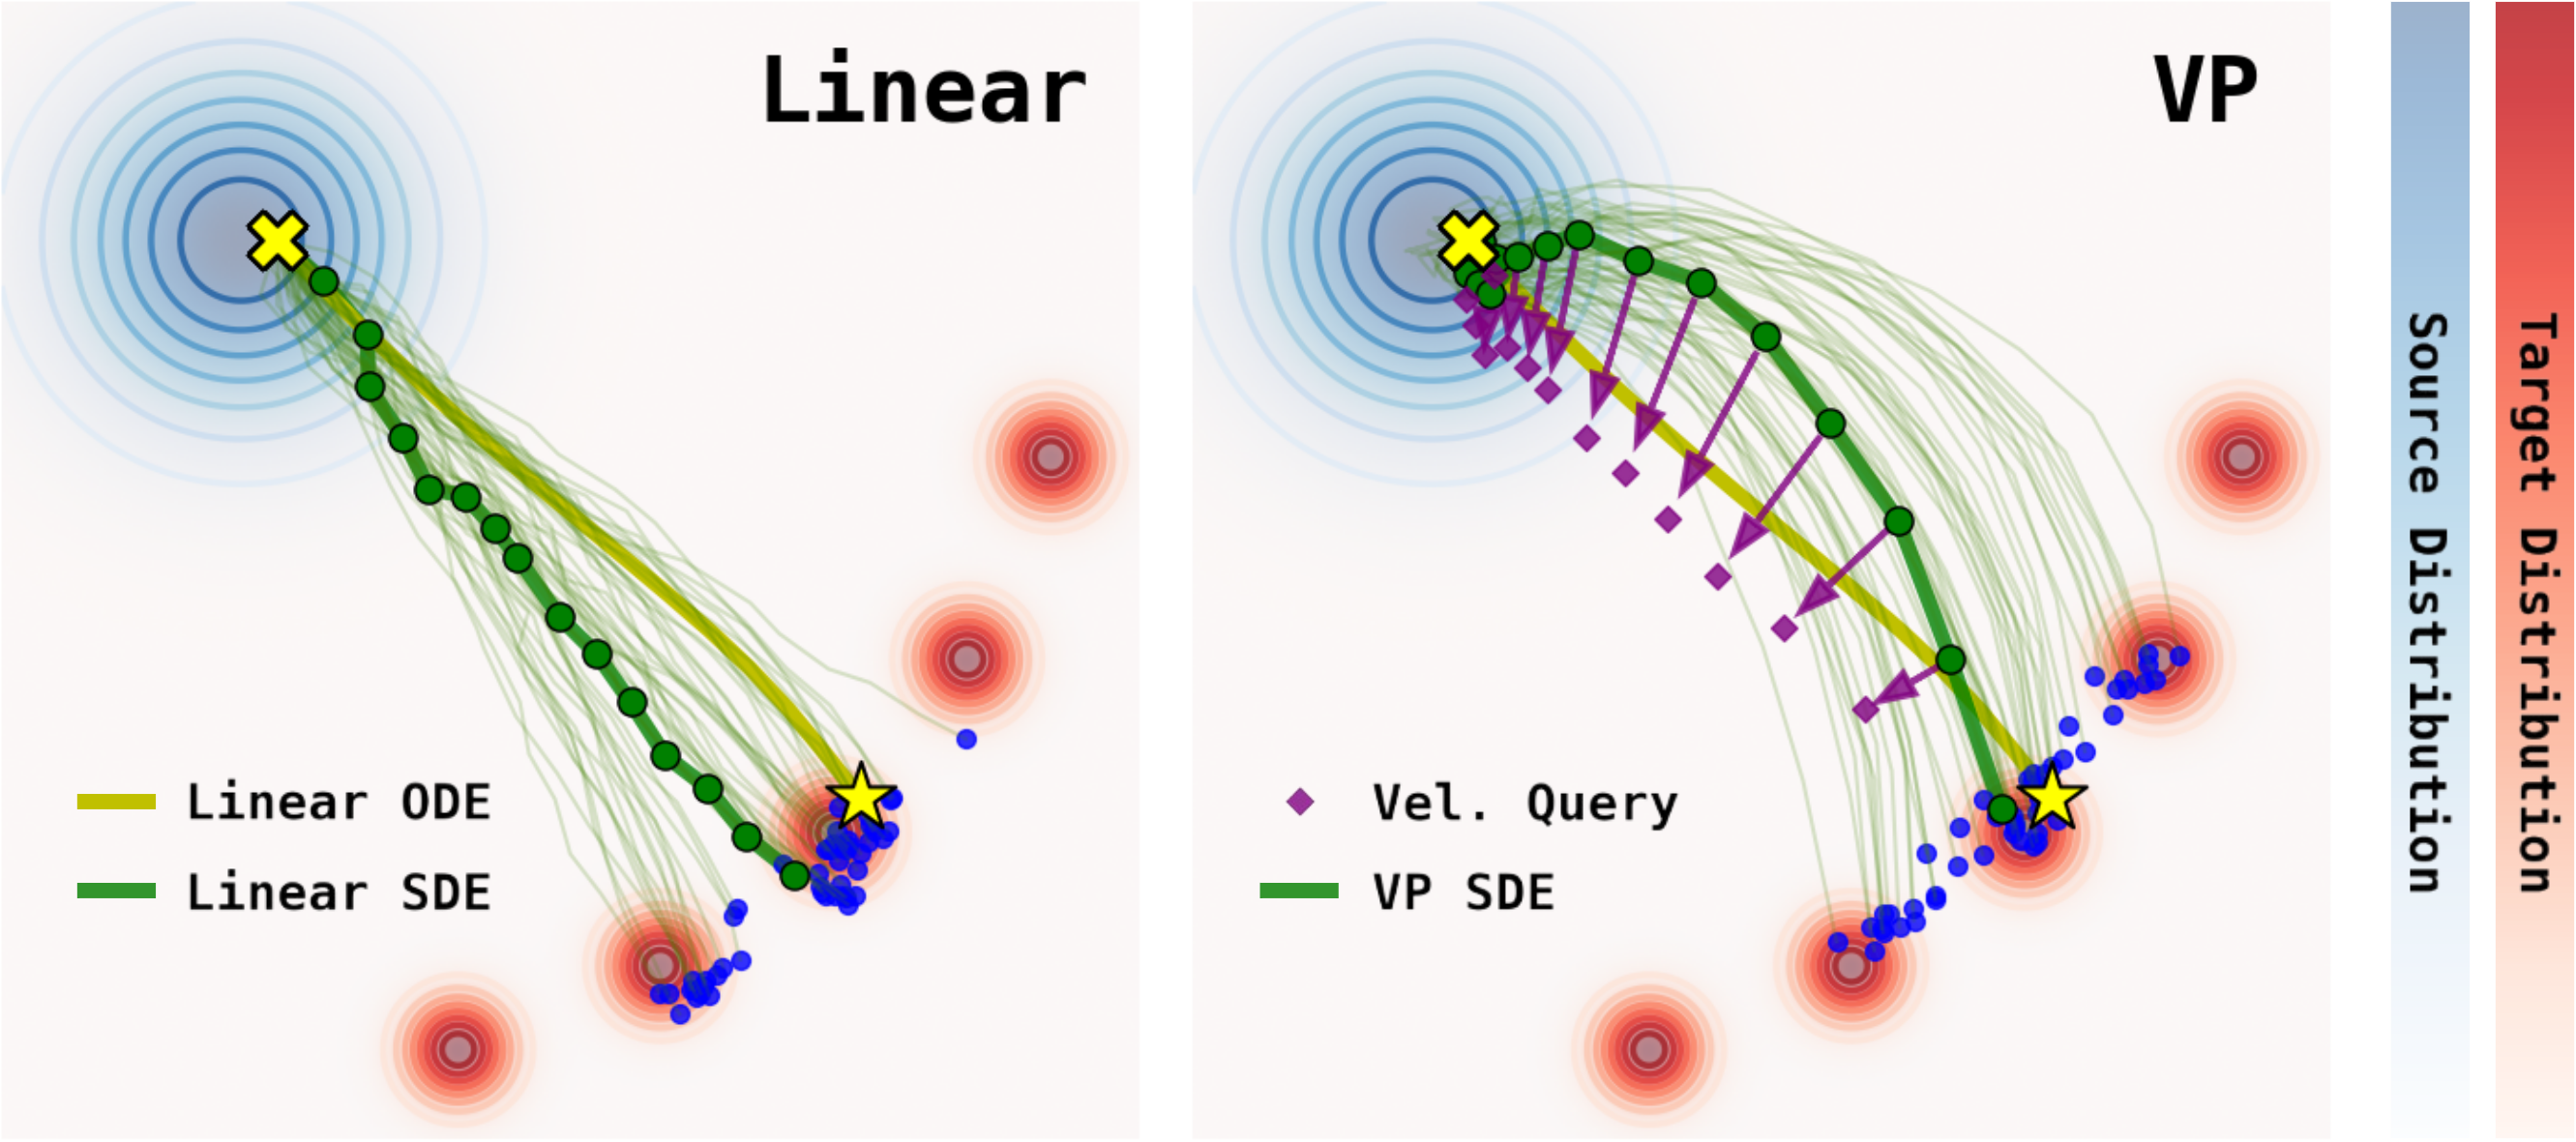
\includegraphics[width=\linewidth]{Figures/ode_sde_toy_visualization/Linear-VP.PNG}
%     \end{minipage}
%     \hfill
%     \begin{minipage}[t]{0.38\linewidth}
%         \small
%         \caption{\textbf{Comparison of Linear-SDE and VP-SDE.} Starting from the same initial noise latent, we generate $50$ samples using Linear-ODE, Linear-SDE, and VP-SDE. The visualization shows how trajectories evolve under different dynamics, highlighting differences in final sample distributions.}
%         \label{fig:ode_sde_viz}
%     \end{minipage}
% \end{figure}


\noindent 
\begin{figure}[t]
    \small
    \centering
    \begin{minipage}[t!]{0.48\linewidth}
        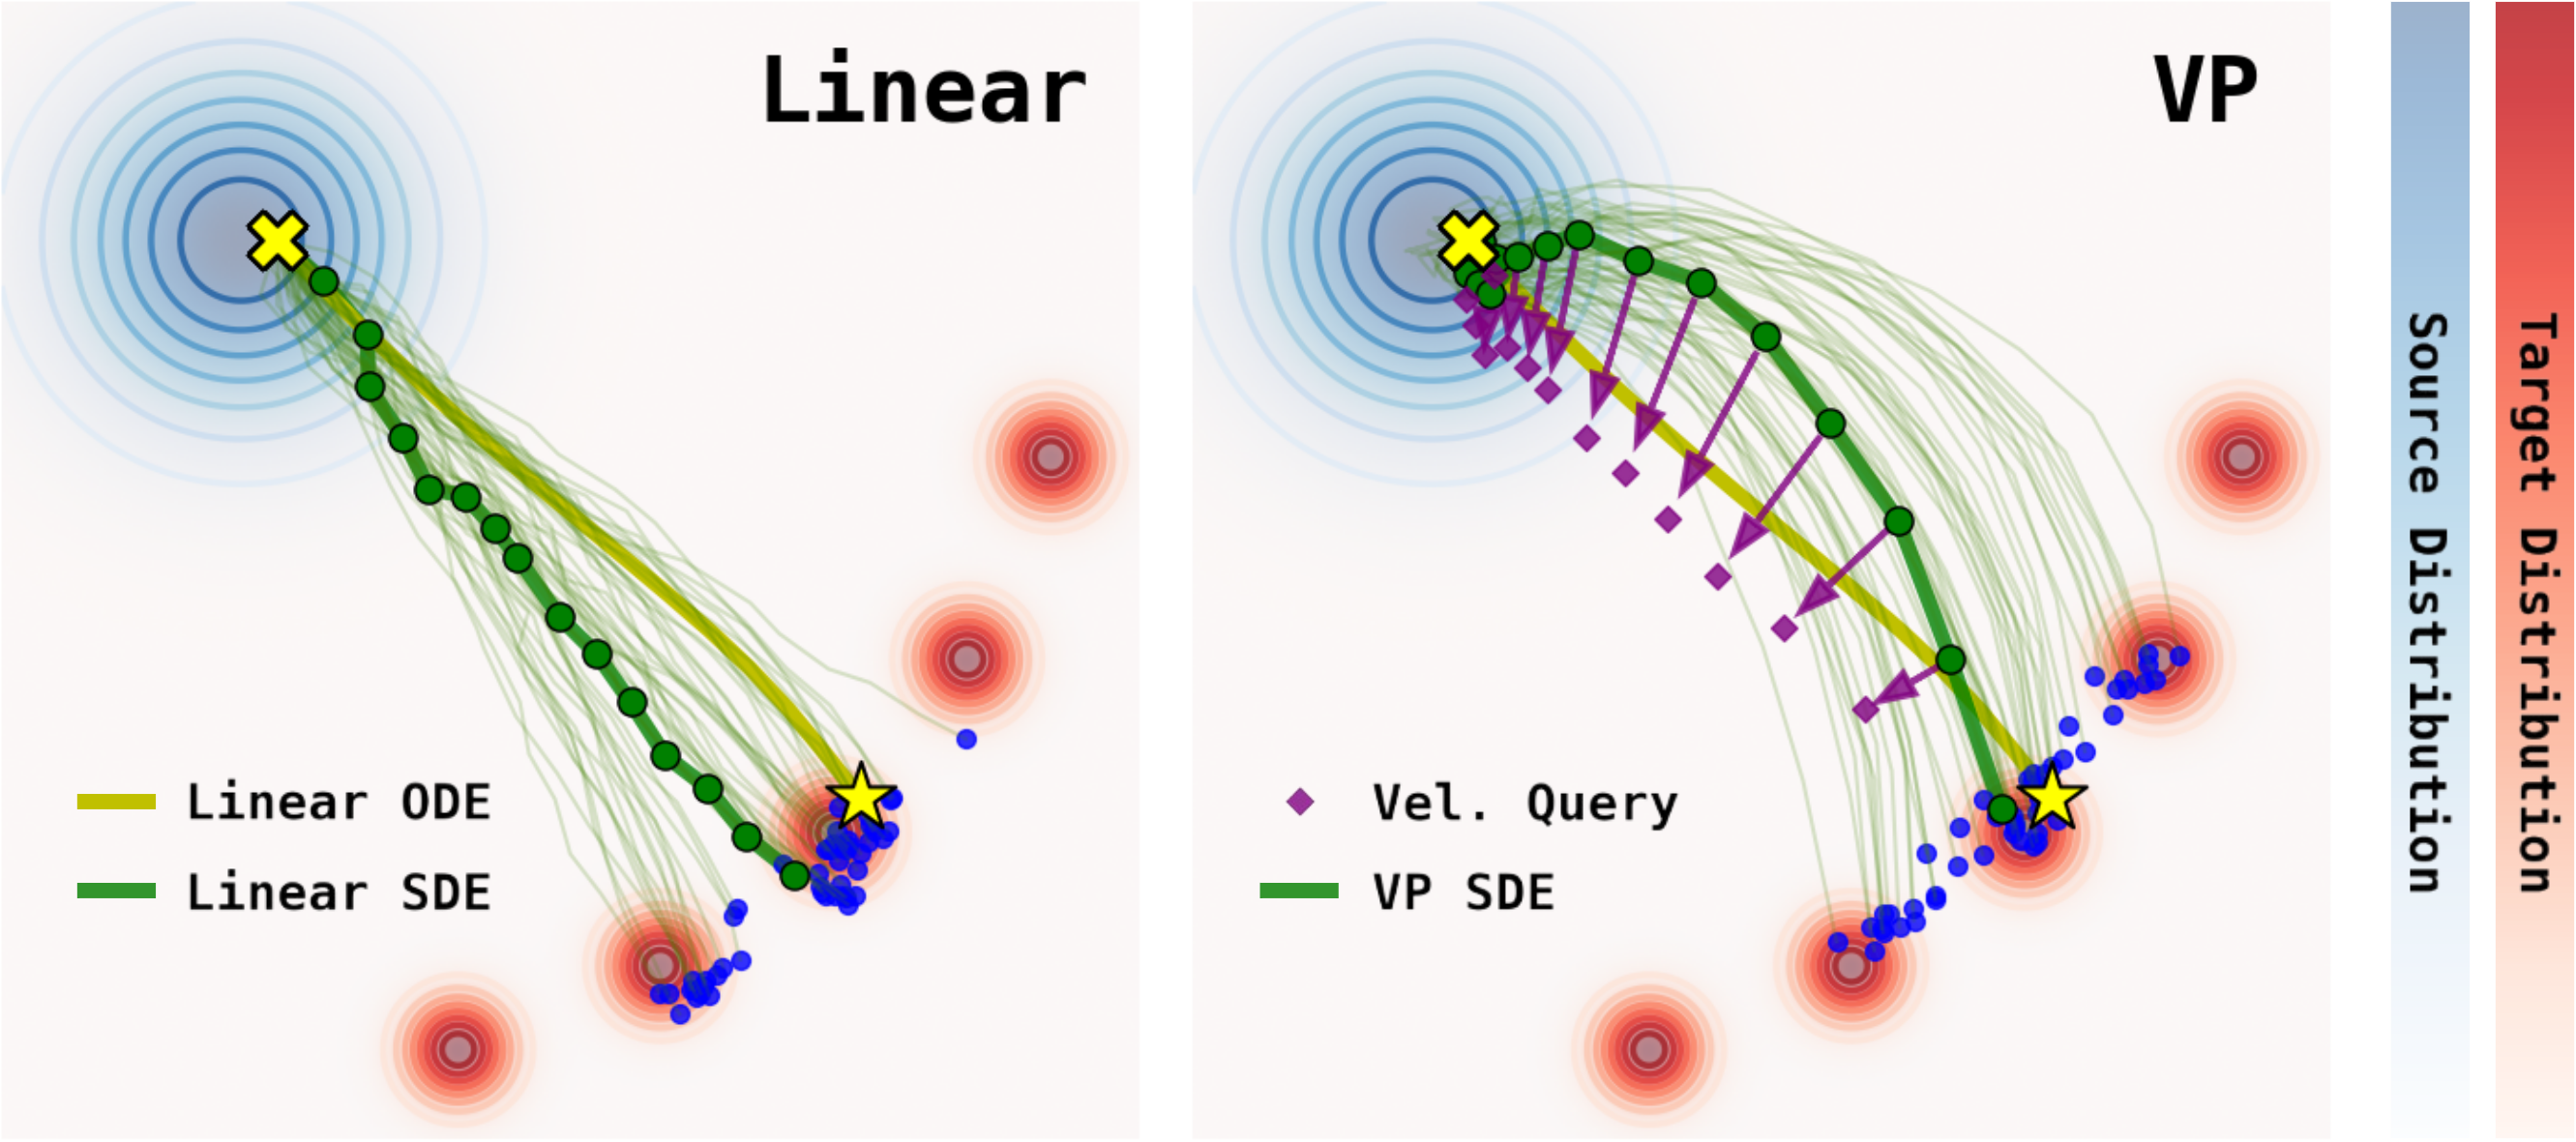
\includegraphics[width=\linewidth]{Figures/ode_sde_toy_visualization/Linear-VP.PNG}
        \caption{
            \textbf{Comparison of Linear-ODE, Linear-SDE, and VP-SDE.}
            The visualization shows how trajectories evolve under different dynamics starting from the same noise latent.
        }
        \label{fig:ode_sde_viz}
    \end{minipage}
    \hfill
    \begin{minipage}[t!]{0.48\linewidth}\vspace{-\topsep}
        {\scriptsize
        \setlength{\tabcolsep}{0.2em}
        \def\arraystretch{0.0}
        \newcolumntype{Z}{>{\centering\arraybackslash}m{0.32\linewidth}}
            \begin{tabularx}{\textwidth}{Z Z Z}
              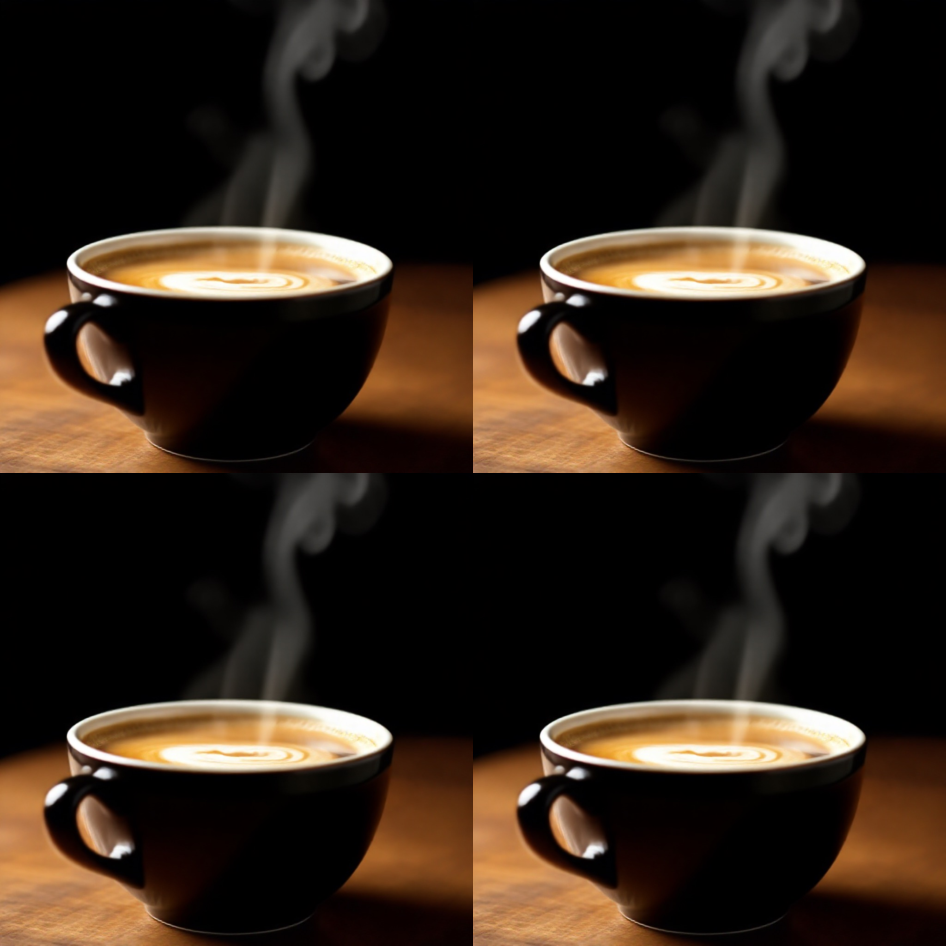
\includegraphics[width=\linewidth]{Figures/variance_test/linear_ode.pdf}
              &  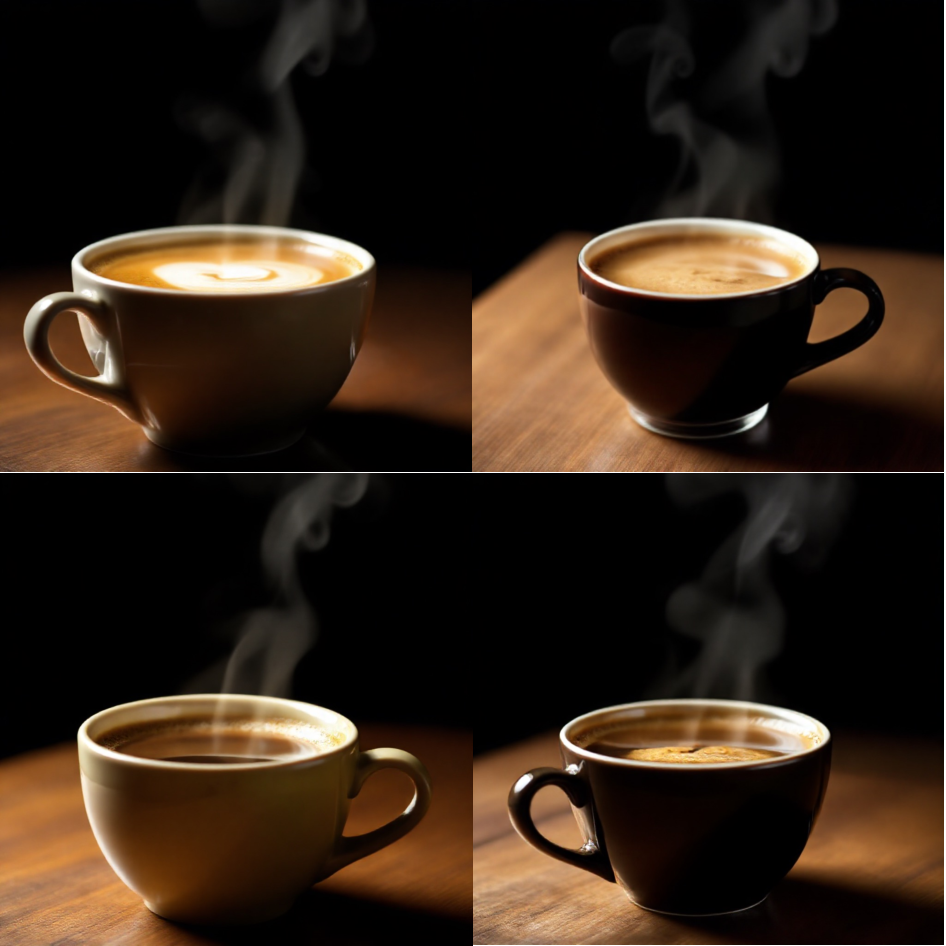
\includegraphics[width=\linewidth]{Figures/variance_test/linear_sde.pdf}
              &  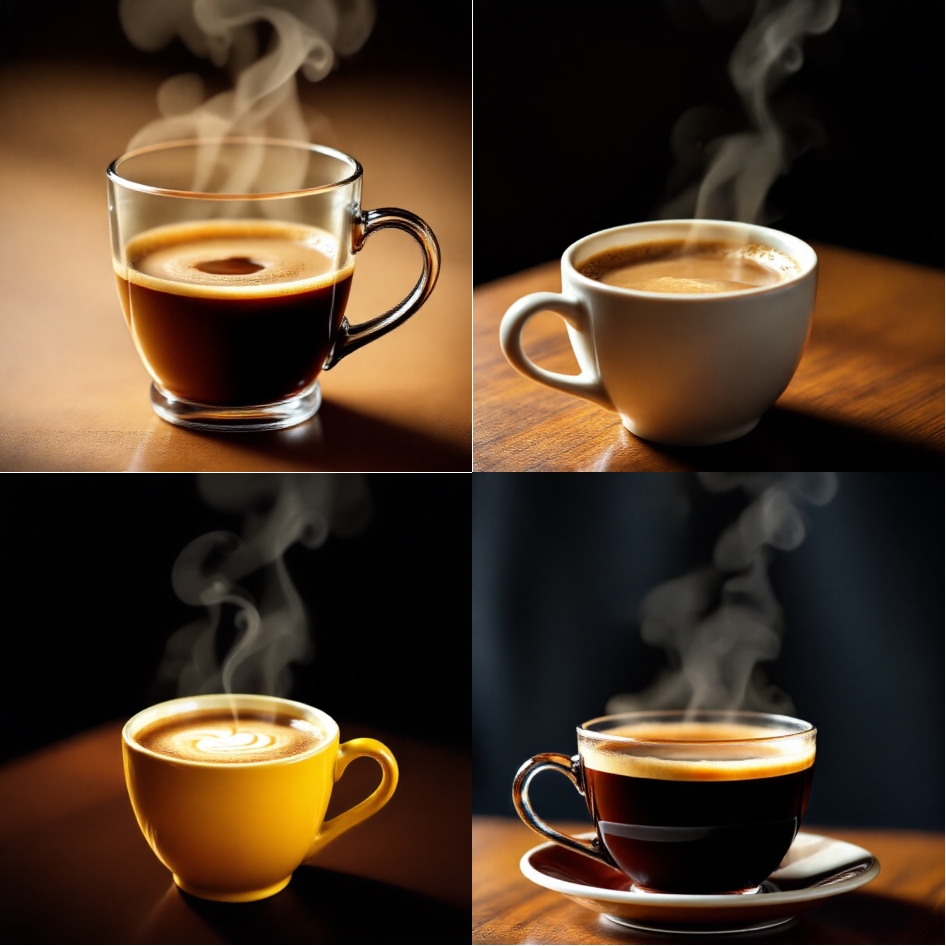
\includegraphics[width=\linewidth]{Figures/variance_test/vp_sde.pdf} \\
              \rule{0pt}{3ex} (a) Linear-ODE
              &
              \rule{0pt}{3ex} (b) Linear-SDE
              &
              \rule{0pt}{3ex} (c) VP-SDE \\
            \end{tabularx}
        }
        \captionof{figure}{
            \textbf{Sample diversity test using FLUX~\cite{BlackForestLabs:2024Flux} under linear and VP interpolant.} All samples share the same initial latent. Prompt: \textit{``A steaming cup of coffee''}.
        }
    \label{fig:variance_test}
    \end{minipage}
    \vspace{-1.1\baselineskip}
\end{figure}




% \begin{figure}
%     \centering
%     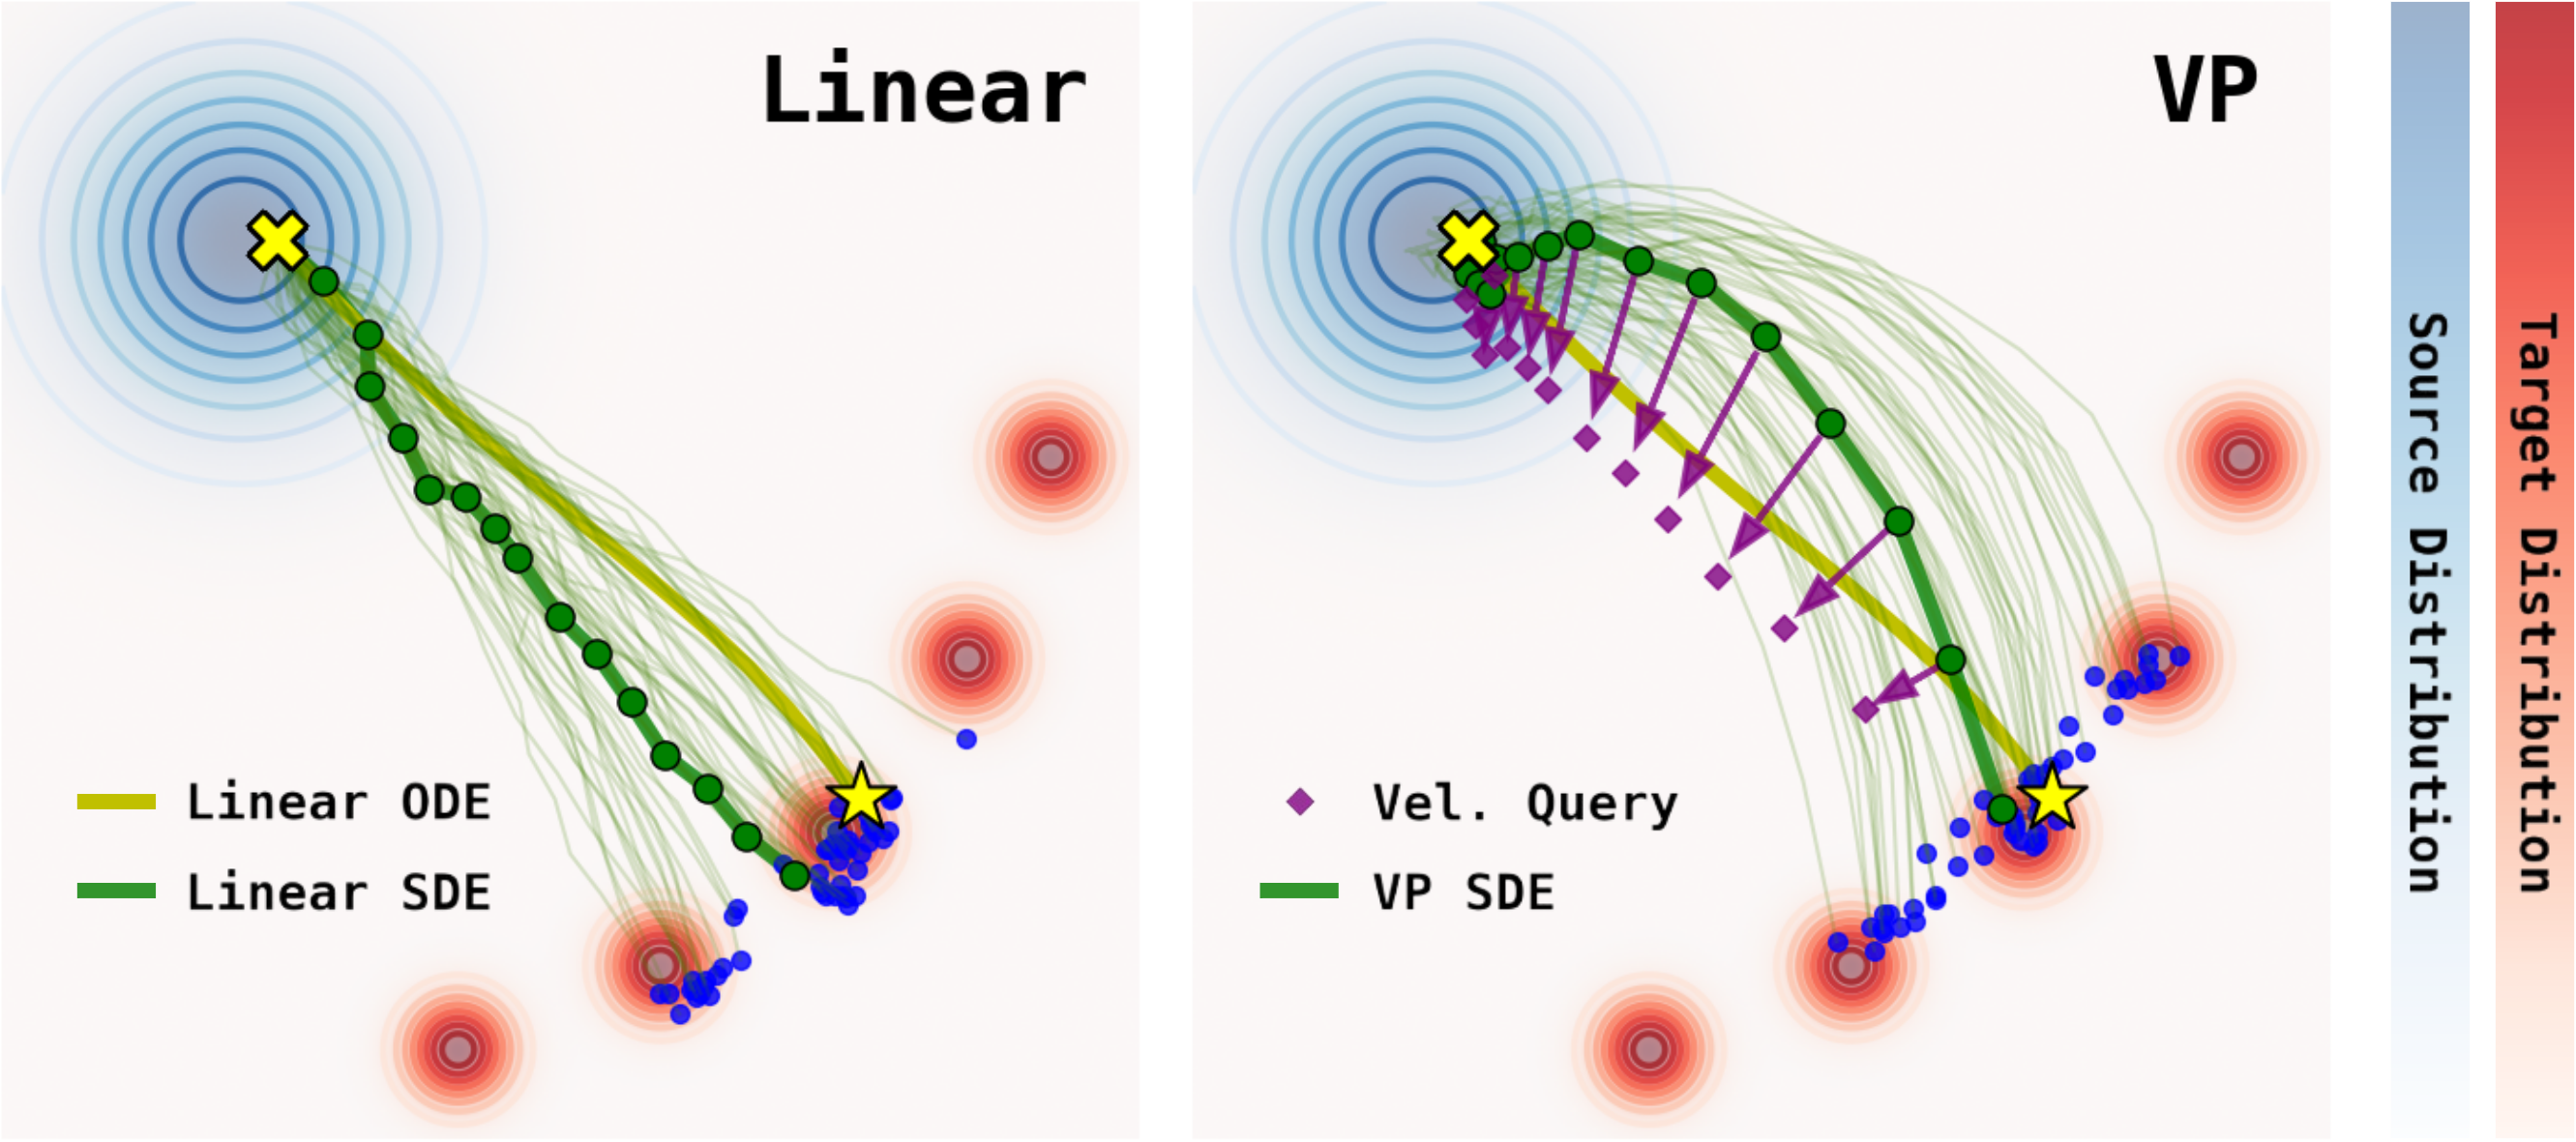
\includegraphics[width=\linewidth]{Figures/ode_sde_toy_visualization/Linear-VP.PNG}
%     \caption{\textbf{Comparison of Linear-SDE and VP-SDE}. Starting from the same initial noise latent, we generate $50$ samples using Linear-ODE, Linear-SDE, and VP-SDE.}
%     \label{fig:ode_sde_viz}
%     \vspace{-1.0\baselineskip}
% \end{figure}



% \begin{table}[!t]
%     \setlength{\tabcolsep}{2.9pt}
%     \centering
%     \small
%     \caption{\textbf{Stochastic interpolant scheduler}. $\beta_t$ is a predefined variance schedule~\cite{DDPM, Score based}.}
%     \label{tab:stochastic_interpolant}
%     % \vspace{-\baselineskip}
%     \newcolumntype{Z}{>{\centering\arraybackslash}m{0.3\linewidth}}
%     \newcolumntype{X}{>{\centering\arraybackslash}m{0.3\linewidth}}
%     \begin{tabular}{X | Z Z}
%         \multicolumn{3}{c}{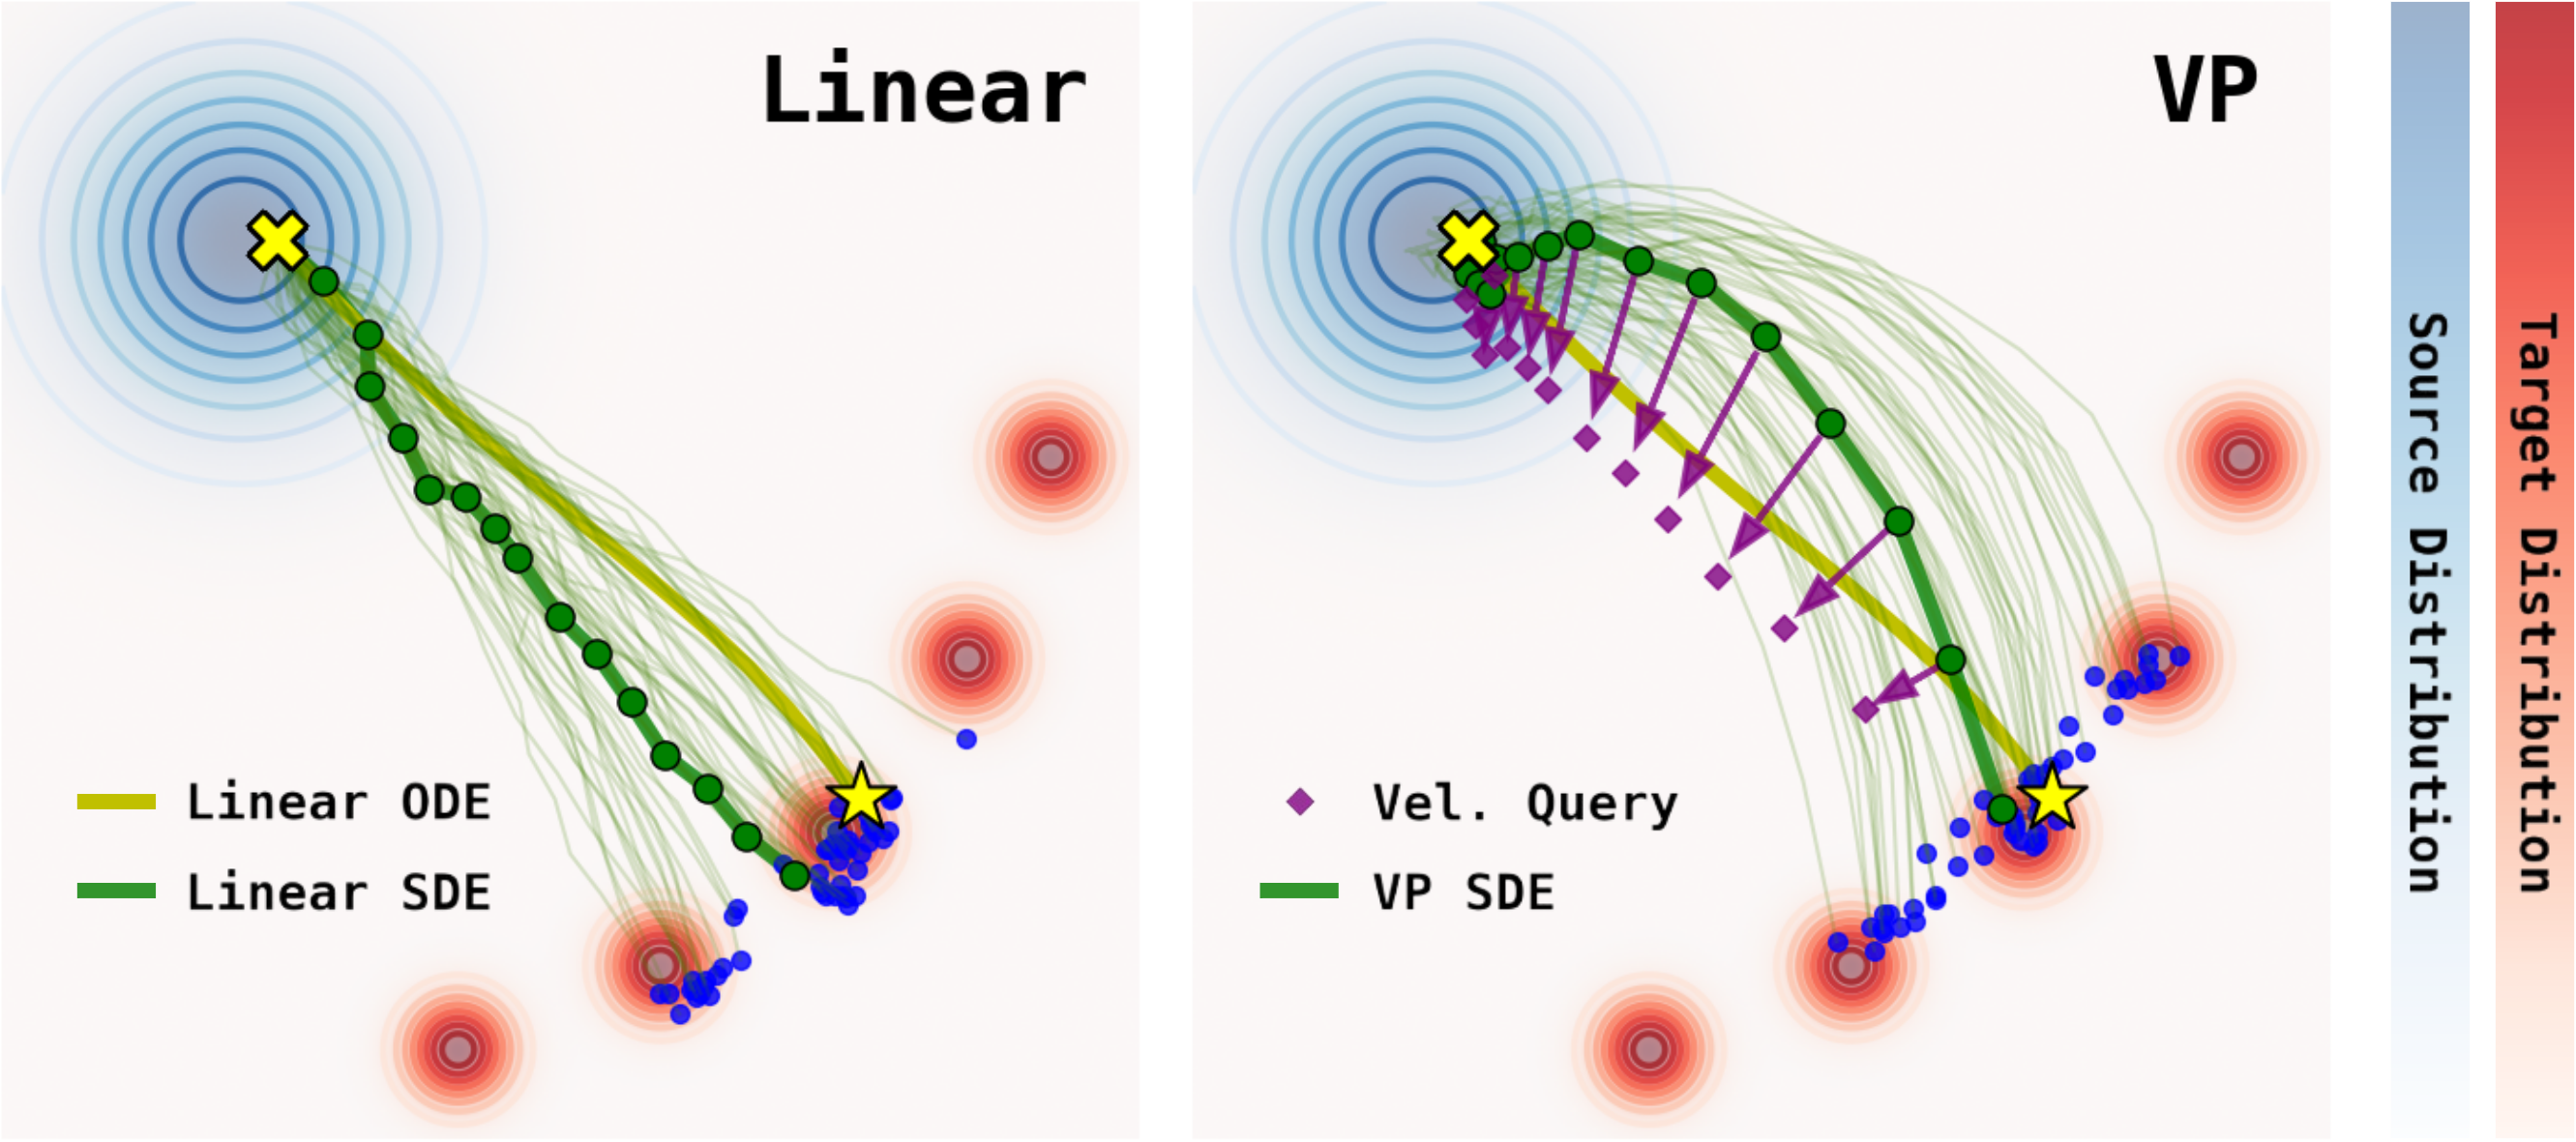
\includegraphics[width=\linewidth]{Figures/ode_sde_toy_visualization/Linear-VP.PNG}} \\
%         \toprule
%         Scheduler & $\alpha_t$ & $\sigma_t$ \\ 
%         \midrule
%         Linear & $1-t$ & $t$ \\
%         \midrule 
%         Variance Preserving & $\exp^{-\frac{1}{2} \int_0^t \beta_s ds}$ & $\sqrt{1 - \exp^{-\int_0^t \beta_s ds}}$ \\
%         \bottomrule
%     \end{tabular}
% \end{table}

\vspace{-1.9\baselineskip}
\section{SDE-Based Particle Sampling in Flow Models}
\vspace{-0.6\baselineskip}
\label{sec:method}
In this section, we review flow and diffusion models within the unified stochastic interpolant framework (Sec.~\ref{sec:stochastic_interpolant}) and introduce our inference-time approaches for efficient particle sampling in flow models (Sec.~\ref{sec:ode_sde_conversion} and ~\ref{sec:scheduler_conversion}). 

\vspace{-0.4\baselineskip}
\subsection{Background: Stochastic Interpolant Framework}
\vspace{-0.5\baselineskip}
\label{sec:stochastic_interpolant}
At the core of both diffusion and flow models is the construction of probability paths $\{ p_t \}_{0 \leq t \leq 1}$, where $\B{x}_t \sim p_t$ serves as a bridge between $\B{x}_1 \sim p_1$ and $\B{x}_0 \sim p_0$:
\begin{align}
    \label{eq:stochastic_interpolant}
    \B{x}_t=\alpha_t \B{x}_0 + \sigma_t \B{x}_1,
\end{align}
where $\alpha_t$ and $\sigma_t$ are smooth functions satisfying $\alpha_0 = \sigma_1 = 1$, $\alpha_1 = \sigma_0 = 0$, and $\Dot{\alpha}_t < 0, \Dot{\sigma}_t > 0$; we denote the dot as a time derivative. This formulation provides a flexible choice of \textit{interpolant} $(\alpha_t, \sigma_t)$ which determines the sampling trajectory. 

\vspace{-0.4\baselineskip}
\subsection{Inference-Time SDE Conversion}
\vspace{-0.5\baselineskip}
\label{sec:ode_sde_conversion}
Flow models~\cite{Lipman:2023CFM, Liu:2023RF} learn the velocity field $u_{t} : \mathbb{R}^d \rightarrow \mathbb{R}^d$, which enables sampling of $\B{x}_0$ by solving the Probability Flow-ODE~\cite{Song:2021SDE} backward in time:
\begin{align}
    \label{eq:pf-ode}
    \mathrm{d} \B{x}_t &= u_{t}(\B{x}_t) \mathrm{d} t.
\end{align}
The deterministic process in Eq.~\ref{eq:pf-ode} accelerates the sampling process enabling few-step generation of high-fidelity samples. However, as discussed in Sec.~\ref{sec:motivation}, the deterministic nature of this sampling process limits the applicability of particle sampling in flow models. 

To address this, we transform the deterministic sampling process into a stochastic process. 
The reverse-time SDE that shares the same marginal densities as the deterministic process in Eq.~\ref{eq:pf-ode}:
\begin{align}
    \label{eq:reverse_sde}
    \mathrm{d} \B{x}_t = \B{f}_t(\B{x}_t) \mathrm{d} t + g_t \mathrm{d} \B{w}, \quad
    % \label{eq:drift_term}
    \B{f}_t(\B{x}_t) = u_{t}(\B{x}_t) - \frac{g_t^2}{2} \nabla \log p_t(\B{x}_t),
\end{align}
where $\B{f}_t(\B{x}_t)$ and $g_t$ represent the drift and diffusion coefficient, respectively, and $\B{w}$ is the standard Wiener process. 
This conversion introduces a noise schedule $g_t$, which can be freely chosen. Although SiT~\cite{Ma2024:sit} arrives at the same conclusion, we provide a more comprehensive proof in Appendix~\ref{sec:appendix_diffusion_coefficient_choice}. 
In our case, we set $g_t = t^2$, scaled by a factor of 3. 
Note that in the case where $g_t=0$ the process reduces to deterministic sampling in Eq.~\ref{eq:pf-ode}.


Using the velocity $u_{t}(\B{x}_t)$ predicted by a pretrained flow model, the score function $\nabla \log p_t(\B{x}_t)$ appearing in the drift coefficient $\B{f}_t(\B{x}_t)$ can be computed as:
\begin{align}
    \label{eq:score_velocity}
    \nabla \log p_t (\B{x}_t) = \frac{1}{\sigma_t} \frac{\alpha_t u_{t}(\B{x}_t) - \dot{\alpha}_t \B{x}_t}{\dot{\alpha}_t \sigma_t - \alpha_t \dot{\sigma}_t}.
\end{align}
This enables the conversion of the deterministic sampling to stochastic sampling, which we refer to as inference-time SDE conversion. 
Given the drift coefficient term $\B{f}_t(\B{x}_t)$ and diffusion coefficient $g_t$, the proposal distribution in the discrete-time domain is derived as follows:
\begin{align}
    \label{eq:proposal_dist_sde}
    p_\theta(\B{x}_{t-\Delta t} | \B{x}_t) = \mathcal{N}(\B{x}_t - \B{f}_t(\B{x}_t) \Delta t,\ 
     g_t^2 \Delta t\ \mathbf{I}).
\end{align}
While previous works have proposed converting an SDE to an ODE to improve sampling efficiency~\cite{Karras2022:EDM, Song2020:DDIM, Lu2022:DPM, Song:2021SDE}, the reverse approach—transforming an ODE into an SDE—has received relatively less attention and has primarily focused on improving sample quality~\cite{xu2023restart, Ma2024:sit}. 
To the best of our knowledge, this work is the \emph{first} to explore SDE conversion in flow models specifically to expand the search space of proposal distribution for efficient particle sampling. 

Since flow models utilize the linear interpolant $(\alpha_t = 1 - t, \sigma_t = t)$, we refer to the generative processes of the flow models using Eq.~\ref{eq:pf-ode} and Eq.~\ref{eq:reverse_sde} as Linear-ODE and Linear-SDE, respectively. 
In Fig.~\ref{fig:ode_sde_viz} (left), we visualize the sampling trajectories of Linear-ODE and Linear-SDE. 
The samples generated using Linear-ODE are identical and collapse to a single point, restricting exploration. 
In contrast, Linear-SDE introduces sample variance, allowing for broader exploration and increasing the likelihood of discovering high-reward samples. 

In Fig.~\ref{fig:variance_test}~(a-b), we visualize images sampled from Linear-ODE and Linear-SDE using FLUX~\cite{BlackForestLabs:2024Flux}. 
As discussed previously, the particles drawn from the proposal distribution of Linear-ODE are identical. In contrast, Linear-SDE introduces variation across different particles, thereby expanding the search space for identifying high-reward samples.
In the next section, we introduce \emph{inference-time interpolant conversion}, which further increases the search space.

          
% =====================================================================================

\vspace{-0.4\baselineskip}
\subsection{Inference-Time Interpolant Conversion}
\vspace{-0.5\baselineskip}
\label{sec:scheduler_conversion} 
To further expand the search space of Linear-SDE, we draw inspiration from the effective use of particle sampling in diffusion models, where we identified a key difference: the \textit{interpolant}.
While the forward process in diffusion models follows the Variance Preserving (VP) interpolant $(\alpha_t = \exp^{-\frac{1}{2} \int_0^t \beta_s \mathrm{d}s}, \sigma_t = \sqrt{1 - \exp^{-\int_0^t \beta_s \mathrm{d}s}})$, with $\beta_s$ denoting a predefined variance schedule, flow models adopt a linear interpolant. 


As shown in the previous works~\cite{Lipman2024:flowguide, shaul2023bespoke}, we note that given a velocity model $u_t$ based on an interpolant $(\alpha_t$, $\sigma_t)$ (\eg~linear), one can transform the vector field and generate a sample based on a new interpolant $(\Bar{\alpha}_s, \Bar{\sigma}_s)$ (\eg~VP) at inference-time. 
The two paths $ \Bar{\B{x}}_s = \Bar{\alpha}_s \B{x}_0 + \Bar{\sigma}_s \B{x}_1 $ and $ \B{x}_t = \alpha_t \B{x}_0 + \sigma_t \B{x}_1 $ are connected through scale-time transformation:
\begin{align}
    \label{eq:scale_time_trans}
    \Bar{\B{x}}_s &= c_s \B{x}_{t_s} \quad t_s = \rho^{-1} (\Bar{\rho}(s)) \quad  c_s = \Bar{\sigma}_s / \sigma_{t_s},
\end{align}
where $\rho(t) = \frac{\alpha_t}{\sigma_t}$ and $\Bar{\rho}(s)=\frac{\Bar{\alpha}_s}{\Bar{\sigma}_s}$ define the signal-to-noise ratio of the original and the new interpolant, respectively. The velocity for the new interpolant is given as:
{\small
\begin{align}
    \label{eq:velocity_transform}
    \Bar{u}_s(\Bar{\B{x}}_s) = \frac{\dot{c}_s}{c_s} \Bar{\B{x}}_s & + c_s \dot{t}_s u_{t_s} \left(\frac{\Bar{\B{x}}_{s}}{c_s} \right), \quad 
    \dot{c}_s = \frac{\sigma_{t_s} \dot{\Bar{\sigma}}_s - \Bar{\sigma}_s \dot{\sigma}_{t_s} \dot{t}_s}{\sigma_{t_s}^2} & 
    \quad \dot{t}_s = \frac{\sigma_{t_s}^2 \left( \Bar{\sigma}_s \dot{\Bar{\alpha}}_s - \Bar{\alpha}_s \dot{\Bar{\sigma}}_s \right)}{\Bar{\sigma}_s^2 \left( \sigma_{t_s} \dot{\alpha}_{t_s} - \alpha_{t_s} \dot{\sigma}_{t_s} \right)}.
\end{align}
}%
Plugging the transformed velocity into the proposal distribution in Eq.~\ref{eq:proposal_dist_sde} after computing the score using Eq.~\ref{eq:score_velocity} gives our efficient proposal distribution.
\begin{align}
    \label{eq:vp_sde_proposal}
    \Bar{p}_\theta(\Bar{\B{x}}_{s-\Delta s} | \Bar{\B{x}}_s) = \mathcal{N}\left(\Bar{\B{x}}_s - \left[ \Bar{u}_s(\Bar{\B{x}}_s) - \frac{g_s^2}{2} \nabla \log \Bar{p}_s(\Bar{\B{x}}_s) \right] \Delta s,\ 
     g_s^2 \Delta s\ \mathbf{I}\right).
\end{align}
Since the new trajectory follows the VP interpolant, we refer to this as VP-SDE. 
We visualize VP-SDE sampling in Fig.~\ref{fig:ode_sde_viz}~(right). At inference-time, we query the velocity of the new interpolant from the original interpolant (purple arrow). 
In Fig.~\ref{fig:variance_test}~(c), we visualize the sample diversity under VP-SDE using FLUX~\cite{BlackForestLabs:2024Flux} which generates more diverse samples than Linear-SDE. 
This property of VP-SDE effectively expands the search space, improving particle sampling efficiency in flow models. 
In Sec.~\ref{sec:interpolant_diversity_analysis}, we provide further analysis on how interpolant conversion contributes to sample diversity. 


Previous works focused on interpolant conversion that enables stable training~\cite{salimans2022progressive, dhariwal2021diffusion, kingma2021variational} and accelerated inference~\cite{shaul2023kinetic, Karras2022:EDM, shaul2023bespoke}. 
We utilize interpolant conversion to enhance the sample diversity in particle sampling, which has \emph{not} been unexplored before. 
% 
Importantly, while we modify the generative process of flow models to align with that of diffusion models, inference-time scaling with flow models still provides distinct advantages. 
The rectified trajectories of flow models~\cite{Liu:2023RF, liu2024instaflow, BlackForestLabs:2024Flux} allow for a much clearer posterior mean, leading to more precise future reward estimation and, in turn, more effective particle filtering. 
 

% \input{Figures/interpolant_analysis}
\section{Analysis of the Interpolant Conversion and Sample Diversity}
\vspace{-0.5\baselineskip}
\label{sec:interpolant_diversity_analysis}

% ================ Analysis Inset ===============
\begin{wrapfigure}{r}{0.45\textwidth}
\centering
\vspace{-1.2em}
\includegraphics[width=\linewidth]{Figures/linear_vp_cos.png}
\captionof{figure}{\textbf{Interpolant log-SNR.} Dashed lines show a reference SNR and timestep. 
}
\vspace{-2.0em}
\label{fig:interpolant_analysis}
\vspace{-0.5em}
\end{wrapfigure}
% ===============================================

In this section, we analyze how the interpolant conversion affects the variance of the proposal distribution and explain why VP-SDE yields higher sample diversity than Linear-SDE, as illustrated in Fig.~\ref{fig:variance_test}. 
To investigate this behavior, Fig.~\ref{fig:interpolant_analysis} visualizes the log-SNR ($\log(\alpha_t^2/\sigma_t^2)$) of commonly used interpolants including linear and VP across timesteps $t \in (0, 1)$. 

Then consider initializing the Linear-SDE timesteps $\{t_s\}_{0 \le s \le 1}$ using the timestep conversion in Eq.~\ref{eq:scale_time_trans}.
This ensures that the log-SNR of the corresponding latents $\mathbf{x}_{t_s}$ matches that of the VP-SDE latents $\bar{\mathbf{x}}_s$ at each step (see the horizontal dashed line in Fig.~\ref{fig:interpolant_analysis}). 
Under this condition, the proposal distributions of the two processes are expressed as follows:
\begin{alignat}{2}
    \nonumber
    \text{Linear-SDE ($t_s$):} \quad 
    & p_\theta(\B{x}_{t_s - \Delta t_s} \mid \B{x}_{t_s}) 
    &&= \mathcal{N} \left( \B{x}_{t_s} - \B{f}_{t_s}(\B{x}_{t_s}) \Delta t_s,\ g_{t_s}^2 \Delta t_s\ \mathbf{I} \right) \\
    \nonumber
    \text{VP-SDE:} \quad 
    & \Bar{p}_\theta(\Bar{\B{x}}_{s - \Delta s} \mid \Bar{\B{x}}_s) 
    &&= \mathcal{N} \left( \Bar{\B{x}}_s - \Bar{\B{f}}_{s}(\Bar{\B{x}}_{s}) \Delta s,\ 
    g_s^2 \Delta s\ \mathbf{I} \right) = \Bar{p}_\theta(\cdot \mid c_s \B{x}_{t_s}). 
\end{alignat}
% 
Since $\Delta t_s < \Delta s$ at early denoising steps, timestep conversion results in smaller variance $g_{t_s}^2 \Delta t_s$ than VP-SDE for a fixed diffusion coefficient. 
% 
Hence, to match the variance of Linear-SDE ($t_s$) to that of VP-SDE, one can scale the diffusion coefficient to $g'_{t_s} = g_s/c_s \sqrt{\Delta s / \Delta t_s}$. 
% 
Note that this scaling significantly increases the stochasticity at early denoising steps as $c_s \approx 1$ and $\sqrt{\Delta s / \Delta t_s} \gg 1$. 
% 
While this scaling can enhance sample diversity, applying it in isolation injects excessive noise, causing samples to deviate from the predefined denoising trajectory and ultimately degrading output quality. 


In fact, interpolant conversion counteracts excessive noise injection by pairing diffusion coefficient scaling with timestep conversion. 
The two mechanisms act synergistically to increase the sample diversity without harming the sample quality. 
In Sec.~\ref{sec:applications}, we validate this analysis with an ablation study that isolates the effect of each factor. 


\paragraph{Comparison under Identical Timestep and Diffusion Coefficient.}
We next analyze the case where both Linear-SDE and VP-SDE operate under identical, fixed timestep schedules and diffusion coefficients. 
% 
While this setting yields identical proposal distribution variances, Fig.~\ref{fig:interpolant_analysis} shows that the VP interpolant maintains a consistently lower log-SNR, indicating that at any given timestep, VP-SDE samples contain a larger noise component (see the vertical dashed line). 
% 
Consequently, the VP-SDE proposal distribution effectively samples from a noisier latent at each step, resulting in higher sample diversity. 
% 
This reflects the observation that noisier latents produce more diverse samples~\cite{meng2021sdedit}. 
% 
While this work focuses on the interpolant perspective, a systematic exploration of timestep scheduling and diffusion coefficient scaling remains a promising direction for future research. 


% =====================================================================================
\vspace{-0.75\baselineskip}
\section{Rollover Budget Forcing}
\vspace{-0.5\baselineskip}
\label{sec:roll_over}
In the previous sections, we have introduced our inference-time approaches to expand the search space of proposal distribution. Here, we propose a new budget-forcing strategy to maximize the use of limited compute in inference-time scaling. 
To the best of our knowledge, previous particle sampling methods for diffusion models~\cite{Li2024:SVDD, Singh:2025CoDE} employ a fixed number of particles across all denoising steps. 
However, our analysis shows that this uniform allocation may lead to inefficiency, where the NFEs required at each denoising step to obtain a sample $\B{x}_{t-\Delta t}$ with a higher reward than the current sample $\B{x}_t$ significantly varies across different runs. We present the analysis results in Appendix~\ref{sec:appendix_adaptive_time_and_rollover}. 


This motivates us to adopt a \emph{rollover} strategy that adaptively allocates NFEs across timesteps. 
Given a total NFEs budget, the NFEs quota $Q$ is allocated uniformly across timesteps. 
Then at each timestep, if a particle $\B{x}_{t-\Delta t}$ yields a higher reward than the current sample $\B{x}_t$ within the quota, we immediately proceed to the next timestep from the newly identified high-reward sample, rolling over the remaining NFEs to the next step. 
If the allocated quota is exhausted without identifying a better sample, we select the particle with the highest expected future reward from the current set, following the strategy used in SVDD~\cite{Li2024:SVDD}.
The pseudocode of \Ours{} is presented in Appendix~\ref{sec:appendix_inference_time_scaling}. 
In the next section, we demonstrate the effectiveness of~\Ours{}, along with SDE conversion and interpolant conversion. 

